\documentclass[12pt, a4paper, titleauthor, oneside]{mwrep}
%\usepackage{polski}
\usepackage[polish]{babel} 
\usepackage{textcomp}
\usepackage{color}
\usepackage[cp1250]{inputenc}
\usepackage[T1]{fontenc}
\usepackage{listings}
\usepackage{graphicx}


\lstset{
	language=[ANSI]C,
	keywordstyle=\bfseries\ttfamily\color[rgb]{0,0,1},
	identifierstyle=\ttfamily,
	commentstyle=\color[rgb]{0.133,0.545,0.133},
	stringstyle=\ttfamily\color[rgb]{0.627,0.126,0.941},
	showstringspaces=false,
	basicstyle=\footnotesize,
	numberstyle=\footnotesize,
	numbers=left,
	stepnumber=1,
	numbersep=10pt,
	tabsize=2,
	breaklines=true,
	prebreak = \raisebox{0ex}[0ex][0ex]{\ensuremath{\hookleftarrow}},
	breakatwhitespace=false,
	aboveskip={1.5\baselineskip},
   columns=fixed,
   extendedchars=true,
  upquote=true,
 frame=single,
% backgroundcolor=\color{lbcolor},
}



\begin{document}


\pagestyle{empty}
\noindent
\begin{center}
    \Large
    Politechnika Cz�stochowska\\
    Wydzia�u In�ynierii Mechanicznej i Informatyki\\
    Informatyka
\end{center}

\vfill
\vfill
\begin{center}
    \Huge\bfseries
    UDP Chat
\end{center}

\vfill\vfill\vfill
\begin{center}
    \large\bfseries
    Dariusz Synowiec \\
    Dariusz Wilk \\
    Pawel Orlowski \\
\end{center}

\vfill
\begin{center}
\large
    Cz�stochowa, 2010
\end{center}

\cleardoublepage

\pagestyle{headings}

\tableofcontents



\part{Dokumentacja}
\chapter{Wst�p}
\label{cha:wstep}

Program, zgodnie z~nazw�, jest prost� aplikacj� realizuj�c� podstawowe za�o�enia chatu.
Po uruchomieniu programu, wy�wietla si� okno z~czterema polami tekstowymi (patrz Rys. \ref{fig:main}). W~Tytule programu mo�emy zobaczy� do jakiego hosta b�dziemy wysy�a� wiadomo�ci.
 Pierwsze pole tekstowe s�u�y do zmiany hosta docelowego (wystarczy wpisa� ��dany adres i~nacisn�� Enter). Druga kontrolka stanowi list� wiadomo�ci wys�anych i~odebranych w~programie. W~trzecim polu u�ytkownik powinien wpisa� nazw� kt�r� si� identyfikuje. Aby wys�a� komunikat nale�y umie�ci� kursor w~ostatnim polu, wpisa� go i~nacisn�� enter.

 Program wysy�a wiadomo�ci poprzez UDP w~funkcji obs�uguj�cej komunikaty Windows. Odbieranie komunikat�w realizowane jest w~osobnym w�tku. Program nas�uchuje na porcie 13 z~wszystkich adres�w wszelkich komunikat�w i~wy�wietla je w~polu drugim.



\begin{figure}[h]
\centering
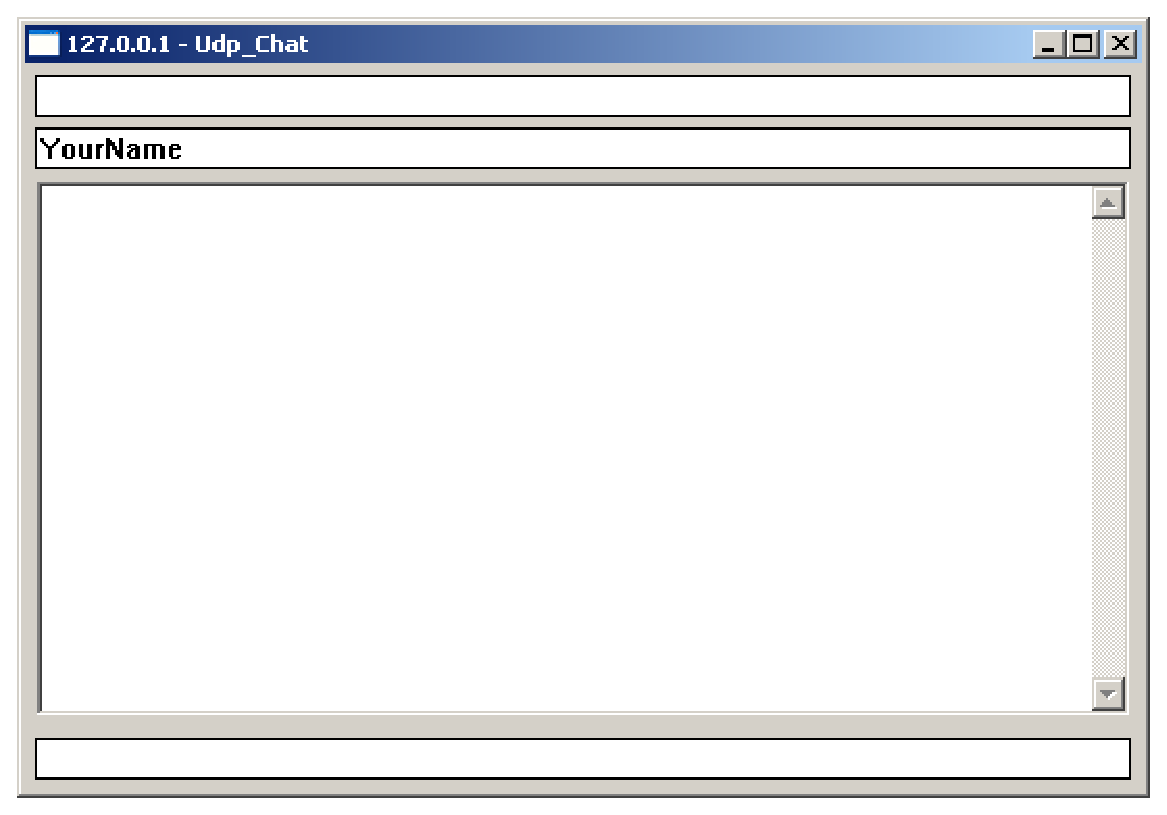
\includegraphics[scale=0.65]{gfx/main}
\caption{G��wne okno programu.}
\label{fig:main}
\end{figure}



\chapter{Wst�p teoretyczny}
\label{cha:protokol_udp}

\section{Protok� UDP}
UDP (ang. User Datagram Protocol) jest jednym z~element�w TCP/IP. Przy pomocy UDP, programy komputerowe mog� wysy�a� komunikaty (zwane datagramami), do innych host�w. UDP jest protoko�em pakietowym, czyli nie wymaga zestawiania specjalnego kana�u komunikacyjnego. 

UDP u�ywa prostej transmisji bez tzw hand-shake. UDP jest zawodny, datagramy mog� dochodzi� w~z�ej kolejno�ci, mog� by� duplikowane lub utracone bez �adnej informacji. Protok� zak�ada, �e korekcja albo nie jest potrzebna albo robiona jest w~aplikacji, unikaj�c dodatkowego nak�adu na obs�ug� interfejsu sieciowego. Aplikacje czasu rzeczywistego cz�sto u�ywaj� UDP, poniewa� dla nich lepiej jest opu�ci� jeden pakiet ni� czeka� na nadej�cie sp�nionego. Gdy korekcja b��d�w jest niezb�dna na poziomie interfejsu sieciowego, aplikacje powinny u�ywa� TCP lub SCTP, kt�re s� w�a�nie do tego celu zaprojektowane.

UDP jest te� u�yteczny dla serwer�w, kt�re musz� odpowiada� ma�� ilo�ci� danych do ogromnej ilo�ci klient�w. Inaczej ni� w~TCP, UDP umo�liwia transmisj� typu broadcast (do wszystkich w~sieci) i~multicast (do wielu host�w).

UDP jest u�ywane przez DNS (Domain Name System), audio/video stream, VoIP (Voice over IP) oraz w~wielu grach.


\section{Porty}

Aplikacje wykorzystuj�ce UDP u�ywaj� socket�w do zestawiania komunikacji pomi�dzy hostami. Sockety dowi�zuj� aplikacj� z~portami serwisowymi, kt�re s�u�� jako ostatnie punkty transmisji danych. Port to struktura j�zyka C~identyfikowana 16-sto bitowym numerem (czyli dozwolone warto�ci pochodz� z~zakresu 0..65535) Port 0 jest zarezerwowany ale jest dozwolone jego u�ycia przez aplikacj� w~przypadku gdy nie spodziewa si� ona odpowiedzi. 

Porty 1 do 1023 s� portami dedykowanymi. Na systemach Unixowych, ��czenie z~tymi portami wymaga praw roota.

Porty 1024 do 49151 to porty zarejestrowane.

Porty 49152 do 65535 u�ywane s� przez aplikacje klienckie do tymczasowych po��cze� z~serwerem.

\section{Protok� IP}
Protok� Internetowy IP (ang. Internet Protocol) jest u�ywany do komunikacji poprzez sie� pakietow�.

IP to g��wnie protok� warstwy Internet Pakietu IP (Internet Protocol Suite) i~ma za zadanie dostarcza� unikalne datagramy (pakiety) z~IP hosta-�r�d�a do komputera docelowego tylko bazuj�c na ich adresach. Do tego celu IP definiuje metody adresowania oraz struktury pakowania datagram�w (pakiet�w). Pierwsza g��wna wersja struktury adresowania, nazywana teraz IPv4, wci�� dominuje w~internecie, pomimo �e jego nast�pca IPv6 jest aktywnie wdra�any na ca�ym �wiecie.


Dane z~warstw wy�szych protoko�u s� pakowane w~pakiety/datagramy. Zestawianie fizycznego po��czenia nie jest potrzebne tu� przed wys�aniem pakiet�w przez jednego hosta do drugiego. IP jest, w~przeciwie�stwie do tradycyjnej telefonii gdzie po��czenie musi by� zestawiane przed ka�d� rozmow�, protoko�em pakietowym (przez co bezpo��czeniowym). 

Dzi�ki abstrakcji jak� oferuje protok�, IP mo�e by� u�ywany w~sieciach heterogenicznych tzn sie� mo�e si� sk�ada� z~Ethernetu, ATM, FDDI, Wi-Fi i~innych. Ka�da warstwa po��czenia mo�e mie� swoj� w�asn� metod� adresowania (lub te� nie mie� jej wcale) oraz analogicznie potrzeb� znalezienia adresu docelowego do zrealizowania po��czenia. Znajdowanie adresu jest realizowane poprzez Protok� Znajdowania Adresu (ang. Adress Resolution Protocol, ARP) dla IPv4 oraz Protok� Odkrywania S�siad�w (ang.  Neighbor Discovery Protocol, NDP) dla IPv6.




\chapter{Kod �r�d�owy}
\label{cha:code}

Ca�y program oparty jest na podstawowych funkcjach dost�pnych w~WinApi oraz bibliotece Winsock. Ca�y program znajduje si� w~pliku \verb|main.cpp|, w~kt�rym znajduj� si� funkcje:
\begin{description}
\item [WinMain] jest g��wn� funkcj� programu przyjmuj�c� standardowe parametry jak dla ka�dego programu okienkowego opartego o~WinApi.
\item [TextWindowProcedure] to funkcja przechwytuj�ca naci�ni�cia przycisk�w. Jest ona u�yta do obs�ugi p�l tekstowych z~adresem hosta i~polem wpisywania wiadomo�ci. Po wykryciu �e w~polu tekstowym naci�ni�ty zosta� jaki� przycisk, wywo�ywana jest funkcja MainWindowProcedure, w~pozosta�ych przypadkach domy�lna procedura obs�ugi okna.
\item [MainWindowProcedure] zawiera ca�� funkcjonalno�� obs�ugi komunikat�w. W~niej interpretowane s� przyci�ni�cia klawisza \verb|Enter| oraz wszystkich pozosta�ych obs�ugiwanych komunikat�w.
\item [ResizeComponents] dba o~to by wszystkie komponenty by�y zawsze prawid�owo rozmieszczone w~oknie nadaj� komponentom rozmiary proporcjonalne do nowej wielko�ci okna.
\item [WinSockInit] inicjuje bibliotek� winsock. Szerzej funkcja opisana jest w~sekcji \ref{ssec:WinSockInit}.
\item [UDPListenerThreadFunction|] to g��wna funkcja w�tku odpowiadaj�cego za nas�uchiwanie. Patrz sekcja \ref{ssec:UDPListenerThreadFunction}.
\item [addressOf] prosta funkcja pobieraj�ca adres IP hosta. Pe�ny opis funkcji w~sekcji \ref{ssec:addressOf}.

%\item [\verb|WinMain|]  jest g��wn� funkc� programu przyjmuj�c� standardowe parametry jak dla ka�dego programu okienkowego opartego o~WinApi.
%\item [\verb|TextWindowProcedure|] to funkcja przechwytuj�ca naci�ni�cia przycisk�w. Jest ona u�yta do obs�ugi p�l tekstowych z~adresem hosta i~polem wpisywania wiadomo�ci. Po wykryciu �e w~polu tekstowym naci�ni�ty zosta�jaki� przycisk, wywo�ywana jest funkcja MainWindowProcedure, w~pozosta�ych przypadkach domy�lna procedura obs�ugi okna.
%\item [\verb|MainWindowProcedure|] zawiera ca�� funkcjonalno�� obs�ugi komunikat�w. W~niej interpretowane s� przyci�ni�cia klawisza \verb|Enter| oraz wszystkich pozosta�ych obs�ugiwanych komunikat�w.
%\item [\verb|ResizeComponents|] dba o~to by wszystkie komponenty by�y zawsze prawid�owo rozmieszczone w~oknie nadaj� komponentom rozmiary proporcjonalne do nowej wielko�ci okna.
%\item [\verb|WinSockInit|] inicjalizuje bibliotek� winsock. Szerzej funkcja opisana jest w~sekcji \ref{ssec:WinSockInit}.
%\item [\verb|UDPListenerThreadFunction|] to g��wna funkcja w�tku odpowiadaj�cego za nas�uchiwanie. Patrz sekcja \ref{ssec:UDPListenerThreadFunction}.
%\item [\verb|addressOf|] prosta funkcja pobieraj�ca adres IP hosta. Pe�ny opis funkcji w~sekcji \ref{ssec:addressOf}.
\end{description}

\section{Zmienne globalne}
\label{sec:globals}

W programie wyst�puje kilka zmiennych globalnych takich jak bufory, numery handle okien, nazwa programu. Spo�r�d nich dwie zmienne globalne dotycz� tematu UDP (patrz Listing \ref{code:globalVariables}):
\begin{description}
  \item[sa] reprezentuje adres IP do kt�rego b�dziemy wysy�a� komunikaty. Zmienna jest typu \verb|sockaddr_in| i~przechowuje:
    \begin{itemize}
      \item rodzin� adresowania (w naszym przypadku jest to AF\_INET), 
      \item numer portu (13)
      \item adres IP (w postaci unii typu \verb|in_addr|).
    \end{itemize}
  \item[soc] przechowuje numer o~socketa, kt�rego u�ywamy do wysy�ania komunikat�w. Jest typu \verb|SOCKET|, co sprowadza si� do \verb|unsigned int|.
\end{description}
Obie zmienne s� globalne poniewa� s� u�ywane w~funkcjach \verb|WinMain| oraz \verb|MainWindowProcedure|. W~pierwszej funkcji obie s� inicjowane. W~drugiej obie s� u�ywane podczas wywo�ania funkcji \verb|sendto|. Dodatkowo zmienna \verb|sa| jest aktualizowana podczas zmiany hosta.

\begin{lstlisting}[caption={globalVariables}, label=code:globalVariables]
struct sockaddr_in sa;
SOCKET soc;
\end{lstlisting}


\section{Funkcje}
Spo�r�d wielu instrukcji zawartych w~funkcjach, opisane zostan� tylko te dotycz�ce komunikacji z~u�yciem protoko�u UDP. Na pocz�tku ka�dej sekcji znajduje si� listing opisywanej cz�ci programu.

\subsection{WinMain}
\label{ssec:winmain}

\begin{lstlisting}[caption={WinMain}, label=code:WinMain]
soc = socket(PF_INET, SOCK_DGRAM, 0);

char  host[200];
sprintf(host, "127.0.0.1");          //loopback

sa.sin_port = htons(13);
sa.sin_family = AF_INET;
sa.sin_addr.s_addr = addressOf(host);
\end{lstlisting}


Linia 1 inicjuje socket w~systemie. U�ywamy rodziny protoko�u PF\_INET. Jako typ transmisji wybieramy SOCK\_DGRAM. Trzeci parametr pozwala sprecyzowa�, kt�ry z~wszystkich dost�pnych protoko��w danego typu w~danej rodzinie chcemy wybra�, podaj�c 0 ��damy domy�lnego protoko�u.


W liniach 3-8 inicjujemy struktur� adresu docelowego. Do zmiennej \verb|host| wpisujemy adres "127.0.0.1" co oznacza interfejs zwrotny. Wszystkie wys�ane pakiety odbierzemy z~powrotem poprzez w�tek nas�uchuj�cy. Wybieramy port 13, rodzin� adresowania AF\_INET. Nast�pnie u�ywamy funkcji \verb|addressOf| by pobra� warto�� numeryczn� adresu IP.



\subsection{MainWindowProcedure}
\label{ssec:mainwindowprocedure}


\begin{lstlisting}[caption={MainWindowProcedure}, label=code:MainWindowProcedure]
DWORD e;
/* send the message */
e = sendto(soc, BuforT, nameLen + dlugoscT + 1, 0, (struct sockaddr *) & sa, sizeof (sa));

if (e == SOCKET_ERROR) {
   MessageBox(hMainWindow, "Sendto Failed", "Error",MB_OK | MB_ICONERROR );
}

...

temp = addressOf(BuforT);
if (INADDR_NONE != temp)
{
   /* change the destination adress */
   sa.sin_addr.s_addr = temp;
   /* update the window title */
   strcat(BuforT, " - ");
   strcat(BuforT, WINDOW_NAME);
   SetWindowText(hMainWindow, BuforT);
}
\end{lstlisting}

Pierwsza cz�� listingu \ref{code:MainWindowProcedure} pokazuje jak realizowane jest wysy�anie komunikat�w to hosta. Po pobraniu tekstu z~pola tekstowego wywo�ywana jest funkcja \verb|sendto| wysy�aj�ca komunikat (BuforT o~d�ugo�ci nameLen + dlugoscT + 1), do hosta (sa), przy u�yciu socketu (soc). Listing \ref{code:sendto} pokazuje deklaracj� funkcji sendo. I~tak:
\begin{description}
  \item[SOCKET s] oznacza numer gniazdka, kt�ry ma zosta� u�yty,
  \item[const char *buf] to wska�nik na bufor z~danymi do wys�ania,
  \item[int len] m�wi o~ilo�ci bajt�w, kt�re maj� by� z~wys�ane,
  \item[int flags] przez ten parametr mo�na przekaza� flagi modyfikuj�ce dzia�anie funkcji,
  \item[const struct sockaddr *to] jest wska�nikiem na struktur� zawieraj�c� adres, port, oraz typ adresowania,
  \item[int tolen] jest d�ugo�ci� (w bajtach) struktury wskazywanej prze \verb|to|.
\end{description}

\begin{lstlisting}[caption={Deklaracja funkcji sendto}, label=code:sendto]
int sendto(
  __in  SOCKET s,
  __in  const char *buf,
  __in  int len,
  __in  int flags,
  __in  const struct sockaddr *to,
  __in  int tolen
);  
\end{lstlisting}

Druga cz�� listingu \ref{code:MainWindowProcedure} zawiera cz�� kodu zmieniaj�c� adres wysy�kowy. Ten kawa�ek programu jest wywo�ywany po naci�ni�ciu klawisz enter w~polu nazwy hosta. W~linii 11 znajduje si� wywo�anie funkcji \verb|addressOf| zwracaj�cej adres IP hosta docelowego w~postaci liczbowej. Je�eli adres zosta� poprawnie znaleziony (linia 12) nast�puje zmiana adresu (linia 15) oraz zmiana tytu�u okna (linie 7-9).


\section{Funkcja WinSockInit}
\label{ssec:WinSockInit}

\begin{lstlisting}[caption={WinSockInit}, label=code:WinSockInit]
int WinSockInit() {
   int retVal = 0;
   WORD version = MAKEWORD(1, 1);
   WSADATA wsaData;

   retVal = WSAStartup(version, &wsaData);

   if (0 != retVal) {
      MessageBox(hMainWindow, "Init Failed", "Error",MB_OK | MB_ICONERROR );
   }

   return retVal;
}
\end{lstlisting}

Funkcja ta ma za zadanie ,,podnie��'' bibliotek� winsock (patrz Listing \ref{code:WinSockInit}). Najpierw wybieramy wersj� 1.1 biblioteki (linia 3). Nast�pnie wywo�ujemy funkcj� \verb|WSAStartup| (linia 6). Gdy nie uda�o si� podnie�� biblioteki, wy�wietlamy stosowny komunikat (linie 8-10).

\subsection{addressOf}
\label{ssec:addressOf}

\begin{lstlisting}[caption={addressOf}, label=code:addressOf]
u_long addressOf(const char * addrStr)
{
   u_long retVal;
   struct hostent* phe;

   char* p1;
   char* p2;

   retVal = inet_addr(addrStr);
   if (INADDR_NONE == retVal)
   {
      phe = gethostbyname(addrStr);

      if (NULL == phe)
      {
         MessageBox(hMainWindow, "Nie znalalem hosta", "Error",MB_OK | MB_ICONERROR );
      }
      else
      {

         p1 = (char *) & retVal;
         p2 = &phe->h_addr[0];

         for (int i=0; i<sizeof(retVal); i++) 
         {
            p1[i]=p2[i];
         }
      }
   }

   return retVal;
}
\end{lstlisting}


Funkcja przyjmuje jako parametr wska�nik na ci�g znak�w zako�czony '\\0', kt�ry stara si� zamieni� na numeryczn� warto�� z~adresem IP. W~linii 9 zak�ada si�, �e w~buforze wej�ciowym znajduje si� adres IP w~gotowej postaci (np ,,127.0.0.1''). Je�eli nie (tzn funkcja \verb|inet_addr| zwr�ci \verb|INADDR_NONE|) wywo�ywana jest funkcja \verb|gethostbyname|. Gdy host zostanie poprawnie znaleziony, adres IP jest kopiowany ze struktury hostent do zmiennej retVal i~zwracany.


\subsection{UDPListenerThreadFunction}
\label{ssec:UDPListenerThreadFunction}

\begin{lstlisting}[caption={UDP server}, label=code:server]
struct sockaddr_in A;
int s, d;

A.sin_family = AF_INET;
A.sin_port = htons(13);
A.sin_addr.s_addr = INADDR_ANY;

s = socket(AF_INET, SOCK_DGRAM, 0);

d = bind(s, (struct sockaddr *) & A, sizeof (A));

...

while(1)
{
  memset(inBuf,0,100);
  d = recvfrom(s, &inBuf[2], 100, 0, (sockaddr *) & A, &dw);

  ...

}
\end{lstlisting}

Pokazana cz�� programu (listing \ref{code:server} w~uproszczeniu pokazuje zasad� dzia�ania tej funkcji. Linie 1-6 inicjuj� struktur� \verb|A| rodzin� adresow� AF\_INET, portem 13. Adresem w~tym przypadku jest INADDR\_ANY (0) co oznacza, �e b�d� przyjmowany komunikaty ze wszystkich adres�w IP (w tym loopback).

Utworzenie nowego socketu odbiorczego (o takich samych parametrach jak socket odbiorczy zadeklarowany wcze�niej) znajduje si� w~linii 8.

W linii 10 jest wywo�anie funkcji \verb|bind| wi���cej socket \verb|s| z~adresem \verb|A|. Po wywo�aniu tej funkcji, nasz program nas�uchuje na sockecie \verb|s| wiadomo�ci przychodz�cych z~adresu \verb|A|.

Linia 14 i~dalsze pokazuj� (obrazowo) jak realizowane jest nas�uchiwanie na porcie. P�tla niesko�czona najpierw czy�ci bufor odbiorczy, nast�pnie wywo�uj� funkcj� \verb|recvfrom|. W�tek tak d�ugo ,,wisi'' w~tej funkcji a� nie otrzyma porcji danych. Z~listingu \ref{code:recvfrom} wida�, �e parametry funkcji s� praktycznie tego samego typu co w~\verb|sentdo| z~t� r�nic�, �e parametry \verb|buf| oraz \verb|from| s� wyj�ciowe.

\begin{lstlisting}[caption={Deklaracja funkcji recvfrom}, label=code:recvfrom]
int recvfrom(
  __in         SOCKET s,
  __out        char *buf,
  __in         int len,
  __in         int flags,
  __out        struct sockaddr *from,
  __inout_opt  int *fromlen
);
\end{lstlisting}





\appendix

\part{Dodatki}
\chapter{Pe�ny listing programu}
\lstinputlisting{main.cpp}



\end{document}

